\section{Discussion}
\label{sec:discussion}
%%
%%
In essence, we propose transformations to the raw data to make it more compressible. The user should choose the right compression technique depending on whether speed or storage is more critical in the query phase. For example, a method with lower compression rate and faster decompression time (such as LZ) may suit interactive visualization applications, while a slower algorithm producing better compression such as BZ2 is more useful for generating static fields and images from very large data. Figure~\ref{fig:spacesaving_lz} and Fig~\ref{fig:spacesaving_bz2} allow us to compare compression rates of the two techniques we have experimented with. As expected, bzip2 provides slightly better compression than LZ at the cost of performance (Table~\ref{tbl:encodingperf}). The user can increase the compression level of bzip2 (1 used) to save more space at the cost of time.

We have presented query performance without the decompression time. This is because our IDV size is 64 times the data size (64 bins used), and the codebook size (about 1\% of the IDV) is smaller than even the raw data. Hence, under the same available resources, either both raw data and codebook can be loaded uncompressed, or both need to be decompressed. When decompression is needed, only a few locations are to be decompressed and read from the codebook of each block. On the other hand, full data blocks, or significant fractions of them are to be decompressed to access the needed data.

%\paragraph*{Number of Templates:} The template creation technique stands on the assumption
%that a very small number of templates is sufficient due to
%self-similarity present in the data and the distributions. We
%investigate if our template creation strategy produces sufficient
%number of templates. We find that for all the datasets, the encoding
%is performed under the desired threshold only with a fraction of the
%number of templates provided, suggesting that the templates indeed
%contain redundancy. If the search threshold is relaxed to expose more
%templates to each block distribution, the number of templates do not
%increase or increase very little.
%%%
%%%%%%%%%%%%%%%%%%%%%%%%%%%%%%%%%%%%%%%%%%
%%% Table begins
%%%%%%%%%%%%%%%%%%%%%%%%%%%%%%%%%%%%%%%%%%
%\begin{table}[!htb]
%	\centering	
%	\renewcommand{\tabcolsep}{0.09cm}
%	\begin{tabular}{|c|c|c|c|}
%		\hline
%		{\small Dataset} & {\small Number of} & {\small Number of} & {\small Average}\\		
%		{\small } & {\small Input Templates} & {\small Templates Used} & {\small L-2 Error}\\		
%		\hline			
%		{\small Plume} & {\small 403} & {\small 147} & {\small 0.000109482}\\
%		{\small Isabel} & {\small 249} & {\small 322} & {\small 0.0000677}\\
%		{\small Combustion} & {\small 269} & {\small 315} & {\small 0.0002293}\\
%		\hline		
%	\end{tabular}
%	\vspace{-0.3cm}	
%	\caption{\label{tbl:domainutil} Utilization of template set T.}
%\end{table}
%%%%%%%%%%%%%%%%%%%%%%%%%%%%%%%%%%%%%%%%%%%%%%%%%%%%
%%% Table ends
%%%%%%%%%%%%%%%%%%%%%%%%%%%%%%%%%%%%%%%%%%%%%%%%%%%%
%%%
%%
%\paragraph*{Time-Varying Data} 
%\label{subsubsec:tv}
%%
For time-varying datasets, we observed that the sub-range histograms coming from subsequent time steps can be indexed with high space-saving using templates from the first time step only. For 29 time steps of solar plume data, the space saving (computed individually for each time step) falls gradually, but stays well above 90\%. This result indicates that the assumption of distributions being similar to each other holds across time steps as well.
%%
%%%%%%%%%%%%%%%%%%%
%% Diagram begins
%%%%%%%%%%%%%%%%%%%
%\begin{figure}[!htb]
%\centering
%	\subfloat{\label{fig:param_d_1}
%	\includegraphics[width = 0.4\linewidth, keepaspectratio = true]{images/eps/results/paramstudy_data_accuracy.eps}}
%	\subfloat{\label{fig:param_d_2}
%	\includegraphics[width = 0.4\linewidth, keepaspectratio = true]{images/eps/results/paramstudy_data_storage.eps}}
%	\caption{Effect of using same template set across multiple time steps on \textbf{(a)} Average encoding error \textbf{(b)} Encoding time and \textbf{(c)} Storage reduction.}	
%	\label{fig:param_data}
%\end{figure}
%%%%%%%%%%%%%%%%%%%
%% Diagram ends
%%%%%%%%%%%%%%%%%%%